

\tikzset{every picture/.style={line width=0.75pt}} %set default line width to 0.75pt        

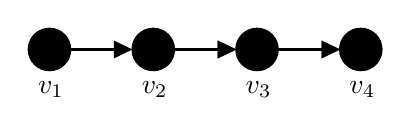
\begin{tikzpicture}[x=0.75pt,y=0.75pt,yscale=-1,xscale=1]
%uncomment if require: \path (0,54); %set diagram left start at 0, and has height of 54

%Shape: Circle [id:dp5966637236046903] 
\draw  [fill={rgb, 255:red, 0; green, 0; blue, 0 }  ,fill opacity=1 ] (10,20) .. controls (10,14.48) and (14.48,10) .. (20,10) .. controls (25.52,10) and (30,14.48) .. (30,20) .. controls (30,25.52) and (25.52,30) .. (20,30) .. controls (14.48,30) and (10,25.52) .. (10,20) -- cycle ;
%Straight Lines [id:da052084780507878126] 
\draw    (20,20) -- (57,20) ;
\draw [shift={(60,20)}, rotate = 180] [fill={rgb, 255:red, 0; green, 0; blue, 0 }  ][line width=0.08]  [draw opacity=0] (8.93,-4.29) -- (0,0) -- (8.93,4.29) -- cycle    ;
%Shape: Circle [id:dp5200693045335503] 
\draw  [fill={rgb, 255:red, 0; green, 0; blue, 0 }  ,fill opacity=1 ] (60,20) .. controls (60,14.48) and (64.48,10) .. (70,10) .. controls (75.52,10) and (80,14.48) .. (80,20) .. controls (80,25.52) and (75.52,30) .. (70,30) .. controls (64.48,30) and (60,25.52) .. (60,20) -- cycle ;
%Straight Lines [id:da33269281061881717] 
\draw    (70,20) -- (107,20) ;
\draw [shift={(110,20)}, rotate = 180] [fill={rgb, 255:red, 0; green, 0; blue, 0 }  ][line width=0.08]  [draw opacity=0] (8.93,-4.29) -- (0,0) -- (8.93,4.29) -- cycle    ;
%Straight Lines [id:da9716435563701427] 
\draw    (70,20) -- (107,20) ;
\draw [shift={(110,20)}, rotate = 180] [fill={rgb, 255:red, 0; green, 0; blue, 0 }  ][line width=0.08]  [draw opacity=0] (8.93,-4.29) -- (0,0) -- (8.93,4.29) -- cycle    ;
%Shape: Circle [id:dp3815536377212252] 
\draw  [fill={rgb, 255:red, 0; green, 0; blue, 0 }  ,fill opacity=1 ] (110,20) .. controls (110,14.48) and (114.48,10) .. (120,10) .. controls (125.52,10) and (130,14.48) .. (130,20) .. controls (130,25.52) and (125.52,30) .. (120,30) .. controls (114.48,30) and (110,25.52) .. (110,20) -- cycle ;
%Straight Lines [id:da660694621597677] 
\draw    (120,20) -- (157,20) ;
\draw [shift={(160,20)}, rotate = 180] [fill={rgb, 255:red, 0; green, 0; blue, 0 }  ][line width=0.08]  [draw opacity=0] (8.93,-4.29) -- (0,0) -- (8.93,4.29) -- cycle    ;
%Straight Lines [id:da23904459539502287] 
\draw    (120,20) -- (157,20) ;
\draw [shift={(160,20)}, rotate = 180] [fill={rgb, 255:red, 0; green, 0; blue, 0 }  ][line width=0.08]  [draw opacity=0] (8.93,-4.29) -- (0,0) -- (8.93,4.29) -- cycle    ;
%Shape: Circle [id:dp3652036582720466] 
\draw  [fill={rgb, 255:red, 0; green, 0; blue, 0 }  ,fill opacity=1 ] (160,20) .. controls (160,14.48) and (164.48,10) .. (170,10) .. controls (175.52,10) and (180,14.48) .. (180,20) .. controls (180,25.52) and (175.52,30) .. (170,30) .. controls (164.48,30) and (160,25.52) .. (160,20) -- cycle ;

% Text Node
\draw (13,34) node [anchor=north west][inner sep=0.75pt]    {$v_1$};
% Text Node
\draw (63,34) node [anchor=north west][inner sep=0.75pt]    {$v_2$};
% Text Node
\draw (113,34) node [anchor=north west][inner sep=0.75pt]    {$v_3$};
% Text Node
\draw (163,34) node [anchor=north west][inner sep=0.75pt]   {$v_4$};


\end{tikzpicture}